% Ch. 02
\chapter{Grammaticalization: characterization and delimitation of the concept} \label{chap:2}

\section{The term ‘grammaticalization’} \label{sec:2.1}

The derivational pattern which the word \textit{grammaticalization} belongs to suggests that it means a process in which something becomes or is made grammatical (cf. \textit{legalization}). In view of this, the term is unfortunate in several respects. Firstly, the term ‘\textbf{grammatical}’ has various meanings. In the above explication of \textit{grammaticalization}, \textit{grammatical} signifies that which belongs to, is part of, the grammar, as opposed to, e.g., what belongs to the lexicon, to stylistics or discourse. Apart from this, \textit{grammatical} has come to mean something completely unrelated to the notion of grammaticalization: \textit{x is grammatical} is an abbreviation of \textit{x is grammatically correct} and accordingly means that x conforms to (as opposed to: is incompatible with, violates) the rules of grammar. What is particularly distressing about this ambiguity is the fact that while \textit{grammatical} may have either meaning in attributive use, it can only have the second meaning in predicative use; and yet the first meaning is needed in the predicative use which is made of it in the above explication of grammaticalization.

Secondly, in addition to the above explication, \textit{grammaticalization} must mean a process in which something becomes or is made  more grammatical (cf. the quotation from Kuryłowicz on Page \pageref{quote:kurylowciz}). We defer to §~6.2 the problem of what it means to say that something belongs to the grammar to a greater or lesser degree, and observe here that this latter notion should be designated by the noun \textbf{grammaticality}. That is, in a theory of grammaticalization, the term ‘grammaticality’ would be needed to mean the degree of grammaticalization which an element has reached. Again, however, this term (or its variant ‘grammaticalness’) is currently based on the other meaning of \textit{grammatical} and therefore means the well-formedness of something according to the rules of grammar.

\label{page11}There would seem to exist a way out. Some authors (e.g. \citet[49]{Givón1975}, \citet[489]{Bolinger1978} have used ‘grammaticization’ instead of ‘grammaticalization’.\footnote{A further abbreviation is represented in Werner's (\citeyear[965f]{Werner1979}) German participle \textit{grammatisiert}, formed on an unattested \textit{grammatisieren} “to grammatize” (i.e. grammaticalize).} We might adopt this use and substitute, accordingly, ‘grammaticity’ for ‘grammaticality’ in the intended sense. Unfortunately, this terminological arrangement would soon come to an inconsistent end, because we would not only have to call ‘grammatic’ what we always have called ‘grammatical’; what is more, this terminological regularization would not be implementable in French, the language in which the term ‘grammaticalization’ was coined in the first place. Finally, it seems paradoxical to give up the well-established ‘grammaticalization’ instead of the rare ‘grammaticization’. We will therefore abide by the terms ‘grammatical’, ‘grammaticality’ and ‘grammaticalization’ and use them exclusively in the sense in which \textit{grammatical} designates that which belongs to the grammar. It seems more convenient to leave the resolution of the terminological conflict to the other side; one might, for example, resort to the expression \textit{grammatically well-formed} if one wants to signify “grammatically well-formed”.

A more serious question is whether the term ‘grammaticalization’ is not unduly stretched if we apply it to such a large range of phenomena. On the one hand, I intend to follow Žirmunskij in subsuming the formation of analytic constructions under grammaticalization. On the other hand, the process does not stop at the level of inflectional morphology. The English pronoun \textit{him}, after having been grammaticalized to a verb-suffixal object marker -\textit{im} in Tok Pisin, has further evolved into an invariable transitive verb marker. Such linear extensions of grammaticalization processes into derivational morphology are not at all rare. On the one hand, since such extensions continue the same pattern, they should be called by the same name. On the other hand, it does not seem correct to say that the suffix -\textit{im}, in its change from an object marker to a transitive verb marker, becomes more grammatical. A term slightly more comprehensive than ‘grammaticalization’ would seem to be needed; but the alternatives that have appeared in the literature are no more satisfactory.\label{page12} \citet{LiEtAL1974}, Givón (\citeyear[209]{Givón1979b}) and Brettschneider (\citeyear[94]{BrettschneiderEtAl1980}) \todo{check the quotes for Givón and Brettschneider} have offered the term ‘condensation’ essentially for what is here called grammaticalization.\footnote{Brettschneider, Li and Thompson actually apply this term only to one specific grammaticalization channel, namely the reduction of a (subordinate) clause to a word.} A precursor of this term is Gabelentz's (\citeyear[433, 436]{Gabelentz1891}) ``Verdichtungsprozess''. In a loose sense, \textit{condensation} may be used to designate one aspect of grammaticalization, namely the narrowing down of the level of grammatical structure (see \sectref{sec:4.3.1}); and this is actually what the above authors have in mind.\label{page12b} However, if we take the word literally, it would have to mean that something becomes denser, compacter in the course of grammaticalization. On the contrary, the authors quoted in \sectref{chap:1} concur that the meaning of a grammaticalized sign is weakened in the same measure as its expression is weakened; a more grammaticalized sign does not say the same thing as a less grammaticalized one in a smaller space, as seems to be implied by the term ‘condensation’.

The term ‘reduction’ (used, for instance, in \citep[103--107]{Langacker1977} does not have this shortcoming, but displays a different one, which, incidentally, it shares with ‘condensation’. It is not specific enough, because it covers also the reduction of a phrase to a compound word, which is not a grammaticalization process.

Authors depending on A. Martinet have sometimes used the term ‘morphématisation’ essentially with the meaning ‘grammaticalization’ (e.g. in \citep[1064f]{Martinet1968}. This presupposes Martinet's terminology, in which ‘morphème’ equals other linguists' ‘grammatical morpheme’. Apart from its local character, ‘morphématisation’ has the disadvantage of being too narrow. Although the formation of grammatical morphemes is probably the focus of grammaticalization, it is by no means all of it.

%\setcounter{page}{1}
We are thus led back to our term ‘grammaticalization’. I see no way to avoid its extension, in a generic sense, to processes such as the one illustrated above. If one wants to make specific reference to just that type of process, one will, of course, not use the term ‘grammaticalization’; §~5.2 will deal with the question of whether a convenient term can be found.

\section{The meaning of ‘grammaticalization’} \label{sec:2.2}

Having settled on the term, we may now characterize more fully the concept. We will first justify one decision which has been presupposed in the above terminological discussion, namely the interpretation of grammaticalization as a process which may not only change a lexical into a grammatical item, but may also shift an item “from a less grammatical to a more grammatical status”, in Kuryłowicz's words. Since adjectives derived in -\textit{al} are commonly non-relative (they have no polar antonyms and do not take part in comparison; cf. \textit{maternal}), one might take the position that the property of being grammatical, of belonging to the grammar, is a binary property and not a matter of degree. As I said, we will postpone discussion of this problem to §~5.2. Anyway, if this were accepted, then grammaticalization could not be a gradual, relative process. From this position it would be correct to say that something is either grammaticalized or not grammaticalized. This is the position of Jakobson, Mel'čuk and Lyons. Lyons writes (\citeyear[234]{Lyons1977}):

\begin{quote}
Different languages make a different selection, as it were, from the set of possible distinctions that could be made and grammaticalize them (i.e. make them grammatically functional) in terms of such categories as tense, number, gender, case, person, proximity, visibility, shape, animacy, etc.
\end{quote}

\noindent Throughout his book, Lyons consistently uses the expression ‘x is grammaticalized in language L’ only if x is a semantic category which is represented by a grammatical category in L. At first sight, this appears to provide us with a simple and intuitively satisfactory interpretation of the notion ‘grammaticalization’. But then we must also provide binary criteria which answer the question:\label{page14b} which conditions must something fulfill in order to be a grammatical category of a language L? Jakobson (\citeyear[489]{Jakobson1959}; see the quotation above on Page \pageref{quote:Jakobson}) and \citet[84]{Mel'čuk1976} answer that the essential criterion is obligatoriness: a meaning is grammatical in L if the speaker cannot choose to leave it unspecified. The criterion of obligatoriness will in fact be used below (\sectref{sec:4.2.3}); but it does not appear to me to be an absolute one. Something is obligatory relative to the context; i.e. it may be obligatory in one context, optional in another and impossible in a third context.\label{page14} Take, for instance, the category of number. In Latin, every noun form compulsorily belongs either to the singular or to the plural; the speaker cannot choose to leave the number unspecified. Here the criterion correctly decides that number is a grammatical category in Latin. In Turkish, most nouns may be specified for number by adding a plural suffix. Some nouns may not, for instance terms of nationality or profession if they form the predicate. No noun may be specified for number if preceded by a cardinal numeral. In most other contexts, number is optional; i.e. the unmarked form may signify the singular or the plural. Is number obligatory in Turkish or not? Certainly not nearly as obligatory as in Latin. Should we therefore say that number is not a grammatical category in Turkish? Would it not be more illuminating to say that number is more grammaticalized in Latin than in Turkish?

An analogous argument could be made with respect to any other criterion that one might be inclined to propose. \sectref{chap:3} will provide abundant evidence that even the mere transition from a lexeme to a grammatical formative (if we were to restrict grammaticalization to this process) is not a leap, but a gradual shift to a new function. The category of prepositions is a notable example. In many languages, there are some prepositions like English \textit{beyond} which need not be treated individually in the grammar because they obey general rules of syntax like other ordinary lexemes; and there are other prepositions like \textit{of} which require special treatment in the grammar because they are obligatory in a number of constructions. The space in between is filled by the bulk of prepositions, which are at different stages on their way from lexeme to grammatical formative. I therefore see no way to avoid the conclusion that grammaticalization is a process of gradual change, and that its products may have different degrees of grammaticality.

If grammaticalization is not a binary, but a gradual change of state, then we must face the problem that it may be an open-ended process. Some authors (e.g. \citet[113--115]{Ronneberger-Sibold1980} have restricted the notion of grammaticalization to the passage from an analytic to a synthetic construction. We have already observed (Page \pageref{Agglutinationstheorie}) that this passage, the agglutination process, stood godfather to the denomination of agglutination theory. Possibly this transition into the unity of the word is the most salient phase of the grammaticalization process. Nevertheless, the nature of the process is the same before and after this phase. The formation of analytic constructions out of ‘word combinations’ (Žirmunskij), on the one hand, and the melting  of an agglutinative to a flexional formation,\footnote{The terminological confusion associated, especially in German, with the term ‘Flexion’ and its cognates may be resolved in English, for our purposes, by the following convention: ‘inflection’ will be opposed to ‘word-formation’ (esp. ‘derivation’) as the syntax-bound part of morphology; ‘flexion’ will be opposed to ‘agglutination’ (and ‘isolation’) as one of the techniques of morphological typology (namely the fusional or amalgamating one, which \citet[129ff]{Sapir1921} calls ‘inflective’). Cf. \citet[41f]{Comrie1981b} on the terminological dilemma.} on the other, are phases of the grammaticalization process. The question naturally arises: where does grammaticalization start, and where does it end? We will provisionally answer this question by diagram \figref{fig:phases}, which incorporates the one presented in \citet[209]{Givón1979b}.

%\setcounter{page}{1}

\begin{figure}
	\resizebox{\textwidth}{!}{
\begin{tabular}{llllllllll}
\lsptoprule

\textsc{level} & {Discourse} & {} & {Syntax} & {} & {Morphology} & {} & {\parbox{2cm}{Morpho\-phonemics}} &  & \\
{} \\
\textsc{technique} & isolating & {{\textgreater}} & {analytic} & {{\textgreater}} & {\parbox{2cm}{synthetic-agglutinating}} & {{\textgreater}} & {\parbox{2cm}{synthetic-flexional}} & {\textgreater} & zero\\
 & {} & {↑} & {} & {↑} & {} & {↑} & {} &  & \\
\textsc{phase} & \multicolumn{9}{l}{~~~~~~syntacticization~~~morphologization~~demorphemicization~~~~~~loss}\\
 & \multicolumn{8}{c}{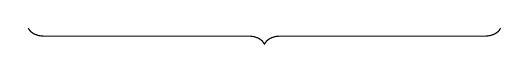
\begin{tikzpicture} \draw[decorate,decoration={amplitude=2mm, brace, mirror}] (0,0) -- (6,0); \end{tikzpicture}}\\
\textsc{process} & \multicolumn{8}{c}{grammaticalization} & \\
\lspbottomrule
\end{tabular}
}
\caption{The phases of grammaticalization} \label{fig:phases}
\end{figure}


\noindent This picture is incomplete and simplified, because it represents only two of the factors involved in grammaticalization, namely those that will be called condensation and coalescence in \sectref{sec:4.3}, and because it pretends a perfect correlation between these two. Nevertheless, it suffices to illustrate, for present purposes, the range of the grammaticalization process and the phases conventionally recognized in it. Thus we assume that grammaticalization starts from a free collocation of potentially uninflected lexical words in discourse. This is converted into a syntactic construction by \textbf{syntacticization}, whereby some of the lexemes assume grammatical functions so that the construction may be called analytic. \textbf{Morphologization}, which here means the same as agglutination, reduces the analytic construction to a synthetic one, so that grammatical formatives become agglutinating affixes. In the next phase, the unity of the word is tightened, as the morphological technique changes from agglutinative to flexional. This transition from morphology to morphophonemics will here be called \textbf{demorphemicization}. Givón calls it lexicalization, and this is the fourth sense in which the term appears in the literature. This need not worry us at the moment. We pass over to the final phase, where expression and content of the grammatical category become zero.

I repeat that this account is simplified. It makes it appear as if the grammaticalization process had a clear-cut end, which we will see it has not. On the other hand, the start of the process is not readily identifiable either, and we will defer this problem, too. The sole function of \figref{fig:phases} is to give a first impression of what is covered by grammaticalization.

A single example to illustrate the whole process is not easy to come by, though such examples probably exist. At any rate, it may be remarked at this juncture that it is not essential to grammaticalization theory that every element affected by grammaticalization enter the process at the start and leave it at the end, where start and end are identified with reference to \figref{fig:phases}. On the contrary, this is certainly the rarest case. I will therefore illustrate a complete grammaticalization process with two examples which together cover the entire range.

From the beginning of the literary tradition up to the postclassical period, the Latin language had an elaborate system of demonstrative pronouns. There was a deictically neutral pronoun \textit{is}, which was also used as an anaphoric personal pronoun. Besides, there were three deictic pronouns, of first (\textit{hic}), second (\textit{iste}) and third (\textit{ille}) person deixis. Apart from their function as \textsc{np}s, which is our concern here, all four could function as determiners. In Archaic Latin, the members of the deictic triad always had some demonstrative force. Their use was subject to no syntactic rule; they occurred where and how the speaker saw fit. However, \textit{ille} was the unmarked member of the triad and began to assume anaphoric function, thus intruding into the area of \textit{is}, which it finally ousted in Vulgar Latin. At this stage, \textit{ille} was a neutral anaphoric pronoun, witness \REF{ex:E1}, from the first half of the 6th cent. \textsc{ad}.

\ea\label{ex:E1}
\langinfo{Latin}{}{~\citep[288]{Pulgram1978}} \\
\textit{duo} rustici sic ad hora captum comederunt, et ita illis contigit, et unus illorum sanguinem deiuso produxit nimium.  (Anth. \textit{obs.cib.} 25)\\
\glt ‘two peasants ate one [turtle dove] just caught, and it so happened to them, and one of them voided too much blood’ \\
\z

\noindent Here we have already entered the path of syntacticization, because the function of \textit{ille} is but the grammatical representation of an \textsc{np} of a previous clause. Still, \textit{ille} is not commonly used as a personal pronoun in subject position. This step has been made, to a varying extent, in the Romance languages. In Standard Italian, for instance, a finite verb does not need an overt subject; \textit{vende} alone may be used to mean ‘he sells’. In French, however, the personal pronoun \textit{il} ({\textless}\textit{ille}) is obligatory if there is no other subject; the corresponding example would be \textit{il vend}. With this, the phase of syntacticization is completed: we have arrived at an analytical verb form.

The morphologization of this combination would presuppose that \textit{il} remains present even when there is a subject in the same clause. This step has not (yet) been taken; but preparations are being made. In a construction such as \textit{Et lui, vend-il des fleurs?}, the left-dislocated \textsc{np} is almost the syntactic subject of the clause, and yet the pronoun \textit{il} cannot be absent.\footnote{Cf. also sentences such as \textit{A quelle heure le train arrive-t-il?, La grammaire n'a-t-elle pas le devoir de s'attacher aux fonctions?, Peut-être les hypothèses contraires veulent-elles seulement dire que ...}} It is enclitic to the verb and could, through agglutination, become a suffixal personal ending. (It is improbable that it will do so in French; but this is not essential to the demonstration.) Summarizing then, we have seen that Latin \textit{ille} has started at the beginning of the scale in \figref{fig:phases} and has advanced, in the shape of French \textit{il}, to the beginning of the morphologization phase.

The second half of this demonstration takes us back to Proto-Indo-European. The so-called secondary personal endings of the active verb were *-\textit{m}, -\textit{s}, -\textit{t} for the three singular persons. Though the details are not recoverable, scholars generally agree that these suffixes derive from the agglutination of personal pronouns. (As will be recalled [Page \pageref{Bopp}], this was already Bopp's position.) In particular, the third person singular suffix *- \textit{t} is most probably a reduced form of the neutral demonstrative stem *\textit{to}{}- (details in \citet[302--305]{Szemerényi1970} and \citet{Seebold1971}. We can therefore be fairly confident that this example takes up at the very point where the former example leaves off.

Still in Proto-Indo-European times, these endings were extended by a suffix *-\textit{i}, whose nature need not concern us here (cf. \pageref{abc}\chk%32
). By the time of Archaic Latin, this -\textit{i} was again lost. The personal suffixes retained their pronominal function, i.e. their capability of representing the subject, over the most part of the subsequent time. Classical Latin \textit{vendit} means ‘he sells’ and needs an overt (pronominal) subject even less than Italian \textit{vende} does. However, the pronominal function gradually got lost, and parallel to this the morphological bond between the stem and the personal endings grew tighter. In Latin, the personal endings cannot be neatly separated from the stem, which means that they are not agglutinative but flexional and they are partly different according to conjugation class; so in this sense, and to this extent, they are demorphemicized. This is the transition from morphology to morphophonemics. The phonological substance of the endings is then further reduced; to the Latin \textit{vendo}, \textit{vendis},\textit{ vendit} corresponds the Italian \textit{vendo}, \textit{vendi}, \textit{vende}. As was mentioned above, the Italian personal endings can still represent, by themselves, the person of the subject. This is no longer so in French. The personal endings have been reduced to zero in the singular (and in the third person plural), which means that apart from exceptions, person is no longer a morphological category of the singular verb. This is the end of the grammaticalization process.

\section{Degrammaticalization}

Various authors (\citet[96]{Givón1975}, \citet[103f]{Langacker1977}, \citet[56--60]{Vincent1980b}) have claimed that grammaticalization is unidirectional; that is, it is an irreversible process, the scale in \figref{fig:phases} cannot be run through from right to left, there is no \textbf{degrammaticalization}. Others have adduced examples in favor of degrammaticalization. The few that have come to my knowledge will be briefly discussed.

\citet[52f]{Kuryłowicz1965} maintains that there is a reverse process to grammaticalization which he calls lexicalization. His examples have, according to him, the following structure: derivational category is grammaticalized to inflectional category and is again lexicalized to derivational category. The examples are: Proto-Indo-European *-\textit{a} was a derivational nominal affix with collective meaning. In Latin, it was grammaticalized to the plural marker of neuter nouns, e.g. \textit{ovum} ‘egg’, pl. \textit{ova}. In Italian, the Latin neuter nouns have become masculine and form their plural in -\textit{i}. However, -\textit{a} is again used as a derivational collective suffix, e.g. in \textit{muro} ‘wall’ — \textit{mura}, \textit{uovo} ‘egg’ — \textit{uova}.

The Pre-English meaning of the perfect was stative. In Modern English, all the verbs which formerly formed their perfect with \textit{be} use \textit{have} now, and the meaning of the perfect is no longer stative but completive. However, for some verbs the perfect with \textit{be} has been restored in the old stative meaning, e.g. \textit{is come}/\textit{gone}.

Again, the verbs \textit{can}, \textit{may}, \textit{shall}, \textit{dare} are original perfect forms (known as preterite-presents in Germanic linguistics). While the perfect has changed its meaning in English, today these forms again signify a present state. Furthermore, the hypothesis that they have changed from inflectional forms to derivational stems is evidenced by the fact that they have developed an inflection of their own: \textit{could}, \textit{might}, \textit{should}, \textit{durst}.\footnote{As a last example, Kuryłowicz mentions in passing the development of sex to gender to sex from Proto-Indo-European via Proto-Germanic to Modern English. This is a process whose details are complicated; however, it is, in the last analysis, an instance of continuous grammaticalization; see \citet[§~7.2]{Lehmann1982b}.}

None of these examples stands up to closer scrutiny. All of them suffer from the defect that the newly evolved derivational category does not possess a minimum of productivity, whereas those Proto-Indo-European derivational categories which they ultimately go back to (if we may assume, for the sake of argument, that perfect was a derivational category in Proto-Indo-European) must clearly have been highly productive, for otherwise they could not have yielded inflectional categories. Instead, the specific examples which Kuryłowicz adduces are virtually the only ones of their kind; that is, they are lexicalized in quite a different sense (the one we already encountered in Žirmunskij): they are frozen, not amenable to any rule, idiomaticized.

Secondly (and this is a difficulty which most putative examples of degrammaticalization are liable to meet with), these lexicalized forms have not really made their way back from a more grammaticalized, inflectional stage, but instead directly continue the original stage. Italian \textit{uova} is not a modern alternative to \textit{uovi}, nor has the construction \textit{is gone} developed on the basis of an earlier \textit{has gone}, nor do \textit{can} etc. go back to older completive perfect forms. Instead, Italian \textit{uova} continues Latin \textit{ova}, and English \textit{is gone} and \textit{can} etc. continue Proto-Germanic stative perfects or preterite-presents, respectively. Finally, although it must be admitted that the -\textit{a} of Ital. \textit{mura} does not go back to Latin, it is not the case that \textit{uova} and \textit{mura} are collectives; they are plural forms. So these examples do not establish a degrammaticalization process.

\citet[122]{Kahr1976} offers a single example of degrammaticalization. Modern Turkish has a postposition \textit{için} ‘for’, which, like some others, takes nominal complements in their unmarked form, but pronominal complements in the genitive (cf. Page \pageref{page39}\chk%71
below). In some rare instances, this morpheme is suffixed, e.g. in \textit{on-un-çün} (d3-\textsc{gen}-for) ‘therefore’. Since these suffixed forms are archaic relics, the modern productive postpositional usage must be explained, according to Kahr, as a degrammaticalization of the suffixal construction.

This is just like explaining the prepositional function of Portuguese \textit{com} ‘with’ through the degrammaticalization of the prefixal construction \textit{comigo}, \textit{contigo} etc. ‘with me, with you’ etc. or, for that matter, of the Latin suffixal construction \textit{mecum}, \textit{tecum} etc. It seems clear that the Turkish case must be just like the Romance one: What was originally an adposition continued to be an adposition in modern times, except in combination with pronouns, where it became affixal already in early times.

%\setcounter{page}{1}
A class of possible examples comes from \textbf{decliticization}. One factor of the phonological weakening of a grammaticalized element is its deaccentuation and subsequent cliticization. If elements could be found which were exclusively clitic at a former stage, but at a later stage allowed an autonomous use, these would be examples of degrammaticalization. \citet[§~3]{JeffersEtAl1980} first adduce the Indo-European relative pronouns *\textit{yo} and *\textit{kwo}{}-, which may be accentuated in their respective Sanskrit and Latin forms \textit{yas} and \textit{qui}. These are said to derive from clitic connective particles which formed a sequence with clitic anaphoric pronouns. Such a sequence coalesced and was reinterpreted as an inflected relative pronoun.

Two objections must be raised against this argument. First, even granting the etymological correctness of this reconstruction, nobody can guarantee that these connectives were actually clitic at the stage in question. Hittite, for instance, does have such sequences as hypothesized by Jeffers and Zwicky; but the connectives are not clitic. Second, the reconstruction proposed by Jeffers and Zwicky is probably false. The syntax of the clitic connectives in the historical languages (e.g. Hittite -\textit{ya}, Sanskrit -\textit{ca}, Latin -\textit{que}) differs markedly from that assumed by them for Indo-European. The relative pronouns are much more plausibly derived from an anaphoric/demonstrative and an interrogative/indefinite pronoun, respectively (see \citealt[Ch. \textsc{vi}.1]{Lehmann1984}), whose relation to the connectives may well be left open. Given the notorious indeterminacy of reconstruction, everything is, of course, possible. What we need, however, are not hypothetical, but historical examples.

Jeffers' and Zwicky's second case is of a completely different nature. The verb of such ancient Indo-European languages as Vedic could be unaccentuated, especially in main clauses; this appears to be no longer possible at later stages. Though this is probably true, it is not an instance of decliticization, since verbs have never been clitic. Clisis is a lexically inherent property of an element which may manifest itself either independently or in dependence on the semantosyntactic context (Jeffers' and Zwicky's “special” vs. “simple” clitics). In the case at hand, however, we are dealing with a certain pattern of sentence intonation which leaves the main verb unaccentuated and which ceases to be usual, or even possible, at a later stage.

The last potential example of degrammaticalization is provided by English. In Proto-Germanic, the genitive suffix -\textit{s} was a flexional ending bound to the word. In Modern English, however, we find such phrases as \textit{the King of England's daughter} and \textit{the man I met yesterday's son}, where the -\textit{s} is agglutinated to a complex \textsc{np}. This looks like a bona fide case. However, the historical details are complex (see \citealt{Janda1980}). On the one hand, the originally flexional -\textit{s} became more agglutinative, in Middle English, as a contingent result of the reduction and regularization of the Old English case paradigm. On the other hand, dialects and lower sociolects of Middle English had the alternative construction ‘\textsc{np} \textit{his} N’ (e.g. \textit{the king (of England) his daughter}) available, which itself became homophonous with the inherited genitive. As a result, the genitive suffix was reanalyzed as a clitic possessive pronoun. Thus, it was not the genitive on its own what expanded to higher syntactic levels. Rather, the (real or putative) clitic possessive pronoun, which had been compatible with these levels from start, got generalized to non-masculine genders.

We may therefore conclude this discussion with the observation that no cogent examples of degrammaticalization have been found. This result is important because it allows us to recognize grammaticalization at the synchronic level. Given two variants which are related by the parameters of grammaticalization to be made explicit in \sectref{chap:4}, we can always tell which way the grammaticalization goes, or must have gone.\footnote{This is true, in the first place, on the synchronic and diachronic axes. The actual historical development may still have deviated from diachronic principles if other factors such as borrowing intervened.} The significance of this for the purposes of internal reconstruction is obvious; see §~8.3.

If grammaticalization is really a unidirectional process, one must ask why this should be so. I will not anticipate here the theoretical considerations of the final chapter, but mention only the explanation that \citet[96]{Givón1975} has given. He says that grammaticalization essentially involves a deletion of both semantic and phonological substance. Degrammaticalization would have to be an enrichment in semantic and phonological substance. Now while the result of a deletion process may be predictable, its source is generally not predictable from the result; so the product of an enrichment process, or of degrammaticalization, would also not be predictable. This appears to be a step in the right direction. However, it remains to be seen, first to what extent the results of grammaticalization processes are really predictable, and secondly, if rules for these processes can be found, why natural languages cannot apply them, at least to non-zero elements, in reverse direction.

\section{Renovation and innovation}

Grammaticalization changes analytic into synthetic constructions. There are, however, numerous instances in the history where languages have changed from the synthetic to the analytic type. This was in fact the observation on which August W. \citet[14--30]{Schlegel1818} based his introduction of the terms ‘analytic’ and ‘synthetic’ in the first place. He observed, for instance, that Latin case inflection has been substituted by prepositional constructions in the Romance languages, that certain tenses are no longer formed by verb inflection but by auxiliaries, and so forth. If such changes from the synthetic to the analytic do occur, aren't they instances of degrammaticalization? This has been maintained by \citet[223--225]{Lightfoot1979}, but the argument has rightly been rejected by \citet[75f]{HeineEtAl1984}. Far from invalidating grammaticalization theory, the evolution synthetic → analytic is predicted by it and has been so predicted since the early days of agglutination theory. If the evolution along grammaticalization scales takes the form of a spiral, this implies that forms which are given up near the end of the scale may be substituted by new forms entering at its beginning. For degrammaticalization to obtain, analytical forms would have to be historical continuants of synthetic forms; but this actually never happens.

This presupposes that we make a clear distinction between the two diachronic relations ‘y continues x’ and ‘y replaces x’. Within a grammaticalization scale, the relation ‘y continues x’ is equivalent to the relation ‘x is grammaticalized to y’. However, the relation ‘y replaces x’ is neither a relation of grammaticalization nor of degrammaticalization. We shall call it, with Meillet's ‘renouvellement’ in mind, the relation of \textbf{renovation}, also called renewal in the literature. Within a grammaticalization scale, ‘y replaces x’ is equivalent to ‘x is renovated by y’. For brevity's sake, I will employ the following symbolism:

%x {\textgreater} y  = ‘x is grammaticalized to y’;
%	
%x /r y  = ‘x is renovated by y’. 
%	
%Examples:
%	
%Latin \textit{ille}        {\textgreater}  French \textit{il}
%	
%Latin \textit{clara mente}  {\textgreater}  Italian \textit{chiaramente}
%
%Latin \textit{ille}        /r  French \textit{ce(lui) là}
%	
%Latin \textit{clare}      /r  Italian \textit{chiaramente}
	
\begin{table}
	\begin{tabular}{lcl}
		\lsptoprule
		x {\textgreater} y & = & ‘x is grammaticalized to y’;\\
		x /r y & = & ‘x is renovated by y’.\\
		\midrule
		\multicolumn{3}{c}{\textsc{examples}}\\
		Latin \textit{ille} &       {\textgreater} &  French \textit{il}\\
		Latin \textit{clara mente} & {\textgreater} &  Italian \textit{chiaramente}\\
		Latin \textit{ille}    &    /r & French \textit{ce(lui) là}\\
		Latin \textit{clare}   &   /r & Italian \textit{chiaramente}\\
		\lspbottomrule
	\end{tabular}
	\todo[inline]{This table is an attempt to make the information more accessible.}
\end{table}	

Further examples are the renovation of the future, perfect, passive and adjective comparison, which had been synthetic categories in the ancient Indo-European languages, by the corresponding analytic categories in several of the modern languages, including English and the Romance languages. A particularly rich field of constant renovation are the subordinating conjunctions as already observed by Meillet. All of these examples will be discussed more fully in \sectref{chap:3}. A wealth of further material for the development of the synthetic towards the analytic may be found in \citet[Ch.~I]{Tauli1966}.

Now consider the situation where an analytic construction y comes into being, but there is no x such that x /r y. For example, the Latin \textit{ille}, \textit{illa} has also been grammaticalized into the French definite articles \textit{le}, \textit{la}. But when we ask what the x is in ‘Latin x /r French \textit{le}, \textit{la}’, we get no answer. Latin had no grammatical category which corresponded to the French articles, so that nothing has been renovated by these. This is an instance of what \citet{Meillet1915} and \citet{Traugott1980} have called (novel) creation. This is an imprecise term, because all linguistic activity, including renovation, is creative activity. ‘\textbf{Innovation}’, as used in \citet{Benveniste1968}, seems to be a better one, because it expresses the desired meaning and provides a suitable contrast to ‘renovation’.\footnote{A wider use of this term has been made in Indo-European linguistics, where it may cover what is here called innovation, renovation and analogical change.} Unfortunately, \textit{to innovate }is intransitive, so that we will resort to \textit{create} in case we need a transitive verb. Further examples of innovation are the introduction of numeral classifiers in Persian, the distinction expressed by \textit{ser} vs. \textit{estar} in Spanish, the progressive form in English and the imperfective vs. perfective aspects in Slavic.

In theory, the distinction between innovation and renovation is entirely clear. Innovation is revolutionary; it creates grammatical categories that had not been in the language before. Renovation is conservative; it only introduces new forms for old categories. The notion of a category which had not been in the language before should cause no problems. Obviously no one would like to commit himself to the claim that no ancestral stage of the Indo-European languages had numeral classifiers, an essence/accidence distinction or a distinction between progressive and neutral or perfective and imperfective aspects. What matters here is the stage immediately preceding the innovation.

In practice, however, there are numerous borderline cases between innovation and renovation. First we must notice that renovation takes its time. There are admittedly cases where the new construction entirely and almost instantly replaces the old one, taking a function and shape maximally similar to the old ones; this has occurred in the renovation of the Latin future in the Romance languages. More often, however, the new and the old constructions coexist for some time. An example is provided by the new analytic and the old synthetic perfect (‘passé composé vs. passé simple’) in the Romance languages. As long as such a situation obtains, the two categories tend to be functionally non-identical, so that we have two categories where we formerly only had one. So far this is not really a conservative change. Conservatism asserts itself only when the old construction falls out of use and the new one takes over its function (and possibly its morphosyntactic form). So what is conservative about renovation is not the particular situation brought about by the introduction of the renovative periphrastic construction, but rather the reentering of a grammaticalization channel which, if run through, will lead to a result maximally similar to the situation which had obtained formerly.

Secondly, two grammatical constructions can be functionally similar only to the extent that they are formally similar. If the renovation of a construction enters upon a path that cannot lead to anything formally similar to the former construction, a complete replacement of the old function will never be obtained, and to this extent the change will be partly renovative, partly innovative. Consider the change that is often called the renovation of Latin case inflection by prepositional constructions. Prepositions will never become case suffixes; even their development into case prefixes is relatively rare (cf. \sectref{sec:3.4.1.3}). Here it suffices to observe that the Latin case suffixes have disappeared, but the Romance prepositions are far from truly fulfilling their function. On the one hand, they do less than that, since strict word order comes in where prepositions (or other means) fail. On the other hand, they do more than that, since prepositions are much more intimately connected with the verb than are case suffixes and may be used to derive compound verbs. Moreover, prepositions can express finer distinctions than cases can because there are more of them. Consequently, the loss of Latin case inflection and the introduction of prepositional constructions is renovative to the extent that the functions of the two constructions overlap, and it is innovative to the extent that they do not.

\section{Reinforcement} \label{sec:2.5}

If an element is weakened through grammaticalization, there are, in fact, two possibilities open to linguistic conservatism. The first is to give it up and replace it by a new, but similar one. This is renovation, as we have just seen. The second is to \textbf{reinforce} it, thus compensating for and checking the decay. Here are some examples: Latin \textit{aliquis} ‘someone’ is reinforced by \textit{unus} ‘one’, yielding *\textit{aliqui-unu}; this is then grammaticalized to Italian \textit{alcuno}, French \textit{aucun} etc. Latin \textit{ille}, which, as we have seen, was grammaticalized to the Romance definite article, was reinforced in its demonstrative function: *\textit{eccu illu} ‘voilà that (one)’ resulted in Italian \textit{quello}. Many Latin prepositions have been reinforced on their way into Romance; e.g. Latin \textit{ante} ‘in front, before’ was strengthened by preposed \textit{ab} ‘from’ before it developed into French \textit{avant}. We will introduce a symbol for the relation of reinforcement: ‘the reinforced form of x is y’ will be written ‘x $\Rightarrow $ y’. The three symbols {\textgreater}, /r, and $\Rightarrow $ will also be used in the converse relations ‘y {\textless} x’, ‘y r/ x’ and ‘y $\Leftarrow $ x’.

Reinforcement can be reiterated ad libitum. For instance, \textsc{ie} *\textit{in} ‘in’ $\Rightarrow $ *\textit{en-tos} {\textgreater} Latin \textit{intus} ‘within, inside’ $\Rightarrow $ *\textit{de-intus} ‘of/from within’ {\textgreater} French \textit{dans} ‘in’ $\Rightarrow $ \textit{dedans} ‘inside’. Pre-Latin *\textit{is} ‘that (one)’ $\Rightarrow $ Latin \textit{iste} ‘that one on your side’ $\Rightarrow $ Proto-Romance *\textit{eccu istu} ‘lo that one’ {\textgreater} It. \textit{questo} ‘this’ $\Rightarrow $ \textit{questo... qui} and French \textit{ce...-ci} ‘this (one) here’. At the stage where the reinforcement is first made, it sounds to puristic ears like a redundant accumulation,\footnote{Cf. the telling remark by A. Schlegel, who was the first to observe some of the above cases; according to him (\citeyear[30]{Schlegel1818}), they “ne laissent pas de sentir un peu la barbarie.”} a hypercharacterization (on the latter, see \citet{Malkiel1957} and \citet[Ch.~\textsc{iv}]{Tauli1966},). But the emphasis soon vanishes, and the reinforced expression becomes neutral again.

The examples illustrate the reinforcement of an element by its morphological union with another one. The situation becomes slightly more complicated when an expression is reinforced not by adding an element next to the grammatical marker already present, but at a different place in the construction. Latin \textit{non} ‘not’ was reinforced by \textit{passum} ‘step’ in a construction *\textit{non} V \textit{passu}, to yield French \textit{ne} V \textit{pas}. The particle \textit{ne} can subsequently be dropped, and the negation \textit{pas} ends up at a different position from Latin \textit{non}. Another example, which I have already used in a simplified manner, but which is really quite complex, are the Latin-Romance prepositions. In Proto-Indo-European, we may assume there were agglutinative case suffixes with rather specific functions. When these got more grammaticalized, they were first specified, and thus reinforced, by adverbs; for example, the accusativus directionis was specified by *\textit{peri} ‘around, along’ {\textgreater} Latin \textit{per} ‘through’. These adverbs were in turn grammaticalized, yielding on the one hand preverbs and on the other adpositions. In Latin we encounter expressions such as \textit{percurrere urbem} or \textit{currere per urbem} ‘to run through the city’. We neglect here the possible hypercharacterization \textit{percurrere per urbem} and pay attention to the fact that in no one of these expressions the suffix is substituted by the preposition or preverb. There is no alternative between case suffix and preposition, such as there is between passé simple and passé composé. We see here that what later on will result in a (partial) renovation, begins as a complex reinforcement (cf. \citealt[55]{Jakobson1936}). In those many instances where the renovative construction starts as an extension of the renovated one, we may speak of \textbf{renovation by reinforcement}; whereas in the other case, where the renovative construction syntagmatically excludes the renovated one, we may speak of \textbf{pure renovation}.

On the same basis, we are led to distinguish between two types of reinforcement: \textbf{simple reinforcement} consists in the morphological union of the bleached element with the specifying one. \textbf{Complex reinforcement} consists in the introduction of a specifying element in a different position of the construction. We started this chapter with simple reinforcement; this is necessarily conservative. In complex reinforcement, however, if the reinforcing element ousts the reinforced one, we have a source of quite novel constructions.\footnote{Developments of this type are also responsible for a considerable amount of headache caused to the historical linguist by certain grammatical formatives. How would we be able to understand the etymology of, e.g., French \textit{pas, rien, point, personne} or of Italian \textit{cosa} ‘what’, if we did not know that they arose through reinforcement (cf. \sectref{sec:3.2.2.3})?} We may even speculate, since no new construction starts ab nihilo, but necessarily uses elements of inherited constructions, that there may be a gradual transition between reinforcement and innovation.\footnote{The distinction between renovation, innovation and reinforcement as made here is also postulated in \citet[115]{Kahr1976}, in the terms 'renewal', 'novel creation' and 'hypercharacterization', respectively.}